%
% main.tex -- Paper zum Thema <circuit>
%
% (c) 2020 Autor, OST Ostschweizer Fachhochschule
%
% !TEX root = ../../buch.tex
% !TEX encoding = UTF-8
%
\chapter{Elektrische Schaltungen
\label{chapter:circuit}}
\kopflinks{Elektrische Schaltungen}
\begin{refsection}
\chapterauthor{Matthias Meyer}
\index{Matthias Meyer}%
\index{Meyer, Matthias}%

%Ein paar Hinweise für die korrekte Formatierung des Textes
%\begin{itemize}
%\item
%Absätze werden gebildet, indem man eine Leerzeile einfügt.
%Die Verwendung von \verb+\\+ ist nur in Tabellen und Arrays gestattet.
%\item
%Die explizite Platzierung von Bildern ist nicht erlaubt, entsprechende
%Optionen werden gelöscht. 
%Verwenden Sie Labels und Verweise, um auf Bilder hinzuweisen.
%\item
%Beginnen Sie jeden Satz auf einer neuen Zeile. 
%Damit ermöglichen Sie dem Versionsverwaltungssysteme, Änderungen
%in verschiedenen Sätzen von verschiedenen Autoren ohne Konflikt 
%anzuwenden.
%\item 
%Bilden Sie auch für Formeln kurze Zeilen, einerseits der besseren
%Übersicht wegen, aber auch um GIT die Arbeit zu erleichtern.
%\end{itemize}

%
% einleitung.tex -- Beispiel-File für die Einleitung
%
% (c) 2020 Prof Dr Andreas Müller, Hochschule Rapperswil
%
% !TEX root = ../../buch.tex
% !TEX encoding = UTF-8
%
\section{Einleitung\label{kettenlinie:section:Einleitung}}
\rhead{Einleitung}
Die Kettenlinie, beschreibt die natürliche Form einer idealen, homogenen und flexiblen Kette, die unter ihrem eigenen Gewicht hängt und an beiden Enden befestigt ist.
Diese Kurve hat in der Mathematik und Physik eine besondere Bedeutung, da sie als Lösung eines Variationsproblems auftritt und die Minimalfläche zwischen zwei Punkten darstellt.
Die Kettenlinie stellt ein Variationsproblem dar, weil sie die Form einer Kurve beschreibt, die eine bestimmte physikalische Bedingung erfüllt: die Minimierung der potenziellen Energie. 


%
% teil1.tex -- Beispiel-File für das Paper
%
% (c) 2020 Prof Dr Andreas Müller, Hochschule Rapperswil
%
% !TEX root = ../../buch.tex
% !TEX encoding = UTF-8
%
\section{Problemstellung\label{kettenlinie:section:Problemstellung}}
\rhead{Problemstellung}
Die Problemstellung der Kettenlinie besteht darin, die Form einer flexiblen, homogenen und nicht dehnbaren Kette zu bestimmen, die an zwei festen Punkten aufgehängt ist und unter dem Einfluss der Schwerkraft hängt.
Mathematisch wird dies als die Suche nach einer Kurve \( y(x) \) beschrieben, die diese Bedingungen erfüllt.
Gegeben für die Problemstellung sind: 
\begin{itemize}
\item
Zwei Aufhängepunkte \( A(x_1, y_1) \) und \( B(x_2, y_2) \).
\item
Eine homogene Kette, d.h., ihre Dichte \( \rho \) ist konstant.
\item
Die Kette ist flexibel und kann sich frei bewegen.
\end{itemize}
Ziel ist es, die Form der Kurve \( y(x) \), welche die Kette zwischen den beiden Punkten annimmt, zu bestimmen.
Wie diese Formel hergeleitet wird, ist im Kapitel \ref{kettenlinie:subsection:Minimum der potenziellen Energie} genauer beschrieben.

\subsection{Mathematische Formulierung
\label{kettenlinie:subsection:Mathematische Formulierung}}
Die potenzielle Energie der Kette wird durch das Integral
\begin{equation}
	U = \int_{x_1}^{x_2} \rho g y \sqrt{1 + (y')^2} \, dx
\end{equation}
beschrieben, wobei \( y' \) die Ableitung von \( y \) nach \( x \) ist und \( g \) die Gravitationskonstante.
Dieses Integral soll minimiert werden, was zur entsprechenden Euler-Lagrange-Gleichung führt.



%%
% teil2.tex -- Beispiel-File für teil2 
%
% (c) 2020 Prof Dr Andreas Müller, Hochschule Rapperswil
%
% !TEX root = ../../buch.tex
% !TEX encoding = UTF-8
%
\section{Herleitung der Balkengleichung
	\label{balken:section:teil2}}
\kopfrechts{Herleitung der Balkengleichung}%
Wir betrachten einen schmalen Balken, welche seine Länge $L$ entlang der $x$-Achse verläuft.
Allfällige Momente wirken um den $y$-Achse im Uhrzeigersinn und erzeugen eine positive Krümmung der Biegelinie $u(x)$ mit der Öffnung gegen oben.
D.h. $u''(x) > 0$.
Dabei verwenden wir die Euler-Bernoulli-Balkengleichung (EBB), die gültig ist, wenn reine Biegung so-wie Querkraftbiegungen auftreten.
Für die EBB werden ausschliesslich Querschnitte betrachtet, die lotrecht zur Nulllinie liegen (im unbelasteten Zustand) \cite{balken:Biegelinie}.

\subsection{Variationsprinzip}
Die Variationsrechnung ist ein Teilgebiet der Analysis, das sich mit kleinen Änderungen in Funktionen und Funktionalen beschäftigt, um Minima und Maxima von Funktionen zu ermitteln. Dabei handelt es sich um mathematische Ausdrücke, die Integrale über eine unbekannte Funktion und ihre Ableitung darstellen können. Ziel ist es, ein Maximum, ein Minimum oder einen Sattelpunkt ausfindig zu machen.

In der Mechanik kommen Variationsrechnungen oft zum Einsatz, da sie die Grundlage aller physikalischen Extremalrechnungen bilden \cite{balken:Variationsrechnung}.

\subsection{Minimalprinzip}
Das Minimalprinzip ist ein Konzept, das besagt, dass ein physikalisches System einen Zustand annimmt, der mit dem geringsten Energieaufwand erreicht wird. In der Physik wird das Minimalprinzip oft formuliert, indem eine minimale Wirkung oder Energie angestrebt wird.

Ein Beispiel hierfür ist eine Feder, die an einem Ende an einer Wand befestigt ist und an ihrem anderen Ende eine Masse trägt. Zieht man die Masse nach unten und lässt sie los, nimmt sie eine Position ein, bei der die potenzielle Energie minimal ist.

Das Minimalprinzip in Bezug auf die Balkengleichung ist ein grundlegendes Konzept der Mechanik, auch bekannt als das Prinzip von Hamilton. Es besagt, dass ein System den Gleichgewichtszustand annimmt, bei dem die potenzielle Energie minimal ist. Für einen Balken tritt dieser Zustand ein, wenn alle äusseren Kräfte, Momente, inneren Beanspruchungen sowie Verformungen des Balkens im Gleichgewicht stehen. Die Anwendung dieses Minimalprinzips führt zur Balkengleichung, die die Gleichgewichtsbedingungen des Balkens beschreibt. 

\subsection{Herleitung der Balkengleichung aus dem Variationsprinzip}
Die Verformungen des Balkens aufgrund der auftretenden Biegespannungen $\sigma_x$ werden durch
\begin{equation*}
	\sigma_x = \frac{E}{\varrho} z
\end{equation*}
und
\begin{equation*}
	\sigma_x = \frac{M_y}{I_y} z
\end{equation*}
beschrieben. Setzt man diese beiden Gleichungen gleich, erhält man
\begin{equation*}
	\frac{E}{\varrho} z = \frac{M_y}{I_y} z
\end{equation*}
und kürzt anschliessend $z$ heraus, so bekommt man
\begin{equation*}
	\frac{E}{\varrho} = \frac{M_y}{I_y}.
\end{equation*}
Dividiert man diese Gleichung durch $E$, um $\varrho$ zu isolieren, erhält man die Formel für den Krümmungsradius
\begin{equation*}
	\frac{1}{\varrho} = \frac{M_y}{E I_y} = \kappa.
\end{equation*}

Bei Biegungen, die aufgrund von Querkräften auftreten, ist das Moment veränderlich und hängt von der Position $x$ ab. Dies führt dazu, dass die Krümmung des Balkens bzw. der Biegelinie von der Position $x$ abhängt. Um die Krümmung zu bestimmen, benötigt man den kürzesten Weg zwischen beiden Auflagern des Balkens.
\begin{figure}
	\centering
	\includegraphics[width=0.8\textwidth]{papers/balken/images/teil2/BiegungBalke2.jpg}
	\caption{Darstellung der Biegelinie $y(x)$ mit dem Balken (rot gekennzeichnet) und dessen Auflagern.}
	\label{fig:Darstellung_der_Biegelinie}
\end{figure}

Zuerst berechnet man die Länge einer Geraden auf der Kurve $y(x)$:
\begin{equation*}
	\Delta s = \sqrt{\Delta x^2 + \Delta y^2} \approx \sqrt{1 + y'(x)^2} \cdot \Delta x
\end{equation*}
und danach mit dem Integral die Kurvenlänge $l(y)$:
\begin{equation*}
	l(y) = \int_{x_1}^{x_2} \sqrt{1 + {y'(x)}^2} \, dx.
\end{equation*}

\subsection{Variationsprinzip für die potentielle Energie}
Um das Variationsprinzip auf die Balkengleichung anwenden zu können, betrachtet man die potenzielle Energie des Balkens. Diese setzt sich aus der Biegeenergie sowie der Energie der äusseren Kräfte zusammen. Die potenzielle Energie im Balken wird minimiert, wenn sich das System im Gleichgewicht befindet.
\begin{figure}
	\centering
	\includegraphics[width=0.8\textwidth]{papers/balken/images/teil2/federgesetz.pdf}
	\caption{Veranschaulichung zur Energie im Balken durch das Flächenträgheitsmoment}
	\label{fig:Veranschaulichung zur Energie im Balken durch das Flächenträgheitsmoment}
\end{figure}

Die Energiedichte des Balkens an einem Punkt $x$ ist gegeben durch
\begin{equation*}
	\frac{1}{2} E I \left( \frac{\partial^2 w}{\partial x^2} \right)^2.
\end{equation*}
Hierbei ist $E I$ das Produkt aus dem Elastizitätsmodul und dem Flächenträgheitsmoment $I$, $w(x)$ beschreibt die Durchbiegung des Balkens.

Zusätzlich zur inneren Energie kommt noch die Last $q(x)$, sodass das Funktional der Euler-Bernoulli-Gleichung wie folgt aussieht:
\index{Euler-Bernoulli-Gleichung}%
\begin{equation*}
	\int_0^L \biggl( -\frac{1}{2} \biggl( \frac{\partial^2 w}{\partial x^2} \biggr)^2 + q(x) w(x) \biggr) \, dx.
\end{equation*}

\subsection{Zeitabhängige Durchbiegung}
Für zeitabhängige Durchbiegungen $w(x,t)$ kommt noch ein kinetischer Energieterm hinzu:
\begin{equation*}
	\frac{1}{2} \mu \left( \frac{\partial w}{\partial t} \right)^2.
\end{equation*}

\subsection{Differentialgleichung für $w(x)$}
Die Lagrange-Funktion lautet daher:
\begin{equation*}
	L(x,w,w',w'') = -\frac{1}{2} E I (w'')^2 + q w.
\end{equation*}
Die Ableitungen der Lagrange-Funktion ergeben:
\begin{align*}
	\frac{\partial L}{\partial w} &= q \\
	\frac{\partial L}{\partial w'} &= 0 \\
	\frac{\partial L}{\partial w''} &= -E I w''.
\end{align*}
Da die Lagrange-Funktion eine höhere Ableitung enthält, erweitert sich die Euler-Lagrange-Differentialgleichung zu:
\begin{equation*}
	\frac{\partial L}{\partial w} - \frac{d}{dx} \frac{\partial L}{\partial w'} + \frac{d^2}{dx^2} \frac{\partial L}{\partial w''} = 0.
\end{equation*}
Einsetzen der Ableitungen ergibt
	\begin{align}
		q - \frac{d^2}{dx^2}(E I w'') &= 0 \\
		\Rightarrow w''''(x) &= \frac{q}{E I}.
	\end{align}

\subsection{Krümmung}
Unsere Lagrange-Funktion ist somit:
\begin{equation*}
	L(x,y,y') = \sqrt{1 + {y'}^2}.
\end{equation*}
Die partiellen Ableitung von $L$ sind:
\begin{equation*}
	\frac{\partial L}{\partial y} = 0
\end{equation*}
und
\begin{equation*}
	\frac{\partial L}{\partial y'} = \frac{y'}{\sqrt{1 + {y'}^2}}.
\end{equation*}

Setzt man $y(x)$ ein und leitet nach $x$ ab, ergibt sich:
\begin{equation*}
	\frac{d}{dx} \frac{\partial L}{\partial y'}(x,y(x),y'(x)) = \frac{d}{dx} \frac{y'(x)}{\sqrt{1 + {y'}^2}} = \frac{(1 + {y'(x)}^2 - {y'(x)}^2) y''(x)}{(1 + {y'(x)}^2)^{\frac{3}{2}}}.
\end{equation*}
Dies führt zu:
\begin{equation*}
	\frac{d}{dx} \frac{\partial L}{\partial y'}(x,y(x),y'(x)) = \frac{y''}{(1 + {y'}^2)^{\frac{3}{2}}}.
\end{equation*}
Die rechte Seite davon ist die Krümmung
\begin{equation*}
	\kappa = \frac{1}{\varrho} = \pm \frac{y''}{(1 + {y'}^2)^{\frac{3}{2}}}.
\end{equation*}

Da wir in unserem Fall $w(x)$ als Funktion für die Biegelinie verwenden, müssen wir das Vorzeichen bestimmen. Da ein positives Moment eine Biegung nach unten verursacht, müssen wir ein negatives Vorzeichen verwenden. Somit erhalten wir:
\begin{equation*}
	\kappa=
	\frac{1}{\varrho}=
	-\frac{w''}{\left(1+{w'}^2\right)^\frac{3}{2}}
\end{equation*}
mit
\begin{equation*}
	w'=
	\frac{dy}{dx} 
\end{equation*}
und
\begin{equation*}
	w''=
	\frac{d^2y}{dx^2}
\end{equation*}

$w$ = Funktion der Durchbiegung

$w'$ = Neigung der Durchbiegung

$w''$ = Krümmung

Da wir in der Baustatik den Rechtssystem verwenden, kehren wir die $z$-Achse so, dass nach unten das positive Vorzeichen ist (siehe Abbildung 13.9).
\begin{figure}
\centering
	\includegraphics[width=0.8\textwidth]{papers/balken/images/teil2/BiegungverdrehteAchsen.pdf}
\caption{Abbildung von den verdrehten $z$-Achse und die positive Momenten, welche auf der Biegelinie wirken.}
\label{fig:Abbildung von den verdrehten $z$-Achse und die positive Momenten, welche auf der Biegelinie wirken.}
\end{figure}

Unsere Funktion zeigt eine Krümmung nach links,
durch die Spiegelung an der $z$-Achse ergibt sich
jedoch eine Krümmung nach rechts.
Bei Rechtskrümmungen sind die zweiten Ableitungen kleiner als 0: $w'' < 0$.
Das ergibt
\begin{equation*}
	\kappa=
	-\frac{w''}{\left(1+{w'}^2\right)^\frac{3}{2}}=
	\frac{M_y}{EI_y}.
\end{equation*}
Der Term $w’$ kann vernachlässigt werden, da im Betracht des Hookesche Gesetz nur kleine Verformungen vorliegen.
Daraus ergeben sich Tangentensteigungen von $w' \ll 1$.
\begin{equation*}
	\kappa=
	-\frac{w''}{\left(1+{w'}^2\right)^\frac{3}{2}}=
	-\frac{w''}{\left(1+0\right)^\frac{3}{2}}=
	-\frac{w''}{1}=-w''=
	\frac{M_y}{EI_y}.
\end{equation*}
Daraus ergibt sich:
\begin{equation*}
	w''=
	-\frac{M_y}{EI_y}
\end{equation*}
mit
\begin{equation*}
	\kappa=
	-w''.
\end{equation*}

\subsection{Temperatureinflüsse}
Temperaturunterschiede verursachen Verformungen in der Balkenachse.
\index{Temperatur}%
Daher ist es wichtig, die Krümmung der Biegelinie bei Temperaturänderungen zu berücksichtigen.
Daraus ergibt sich der Formel.
\begin{equation}
	w''=
	-\frac{M_y}{EI_y}-\alpha_{\text{th}}\frac{\Delta T}{h},
\label{balken:l36}
\end{equation}

$α_th$ = thermische Ausdehnungskoeffizient des Balkenmaterials,

$\Delta T$ = Temperaturunterschied,

$h$ = Höhe des Balkens,

$I_y$ = Flächenträgheitsmoment.

Die Formel \eqref{balken:l36} kann auch wie folgt angegeben werden:
\begin{equation*}
	w''''=
	\left(-\frac{M_y}{EI_y}-\alpha_{\text{th}}\frac{\Delta T}{h}\right)''.
\end{equation*}
Bei einem linearen Temperaturverlauf ergibt sich bei der zweiten Ableitung 0:
\begin{equation*}
	w''''=
	\left(-\frac{M_y}{EI_y}\right)''.
\end{equation*}

\subsection{Querkraft}
Die erste Ableitung des Biegemoments ergibt die Querkraft
\begin{equation*}
	\frac{dM}{dx}=
	M'=
	Q.
\end{equation*}
Daraus ergibt sich
\begin{equation*}
	w'''=
	-\frac{Q}{(EI_y)'}.
\end{equation*}
Mit konstanter Biegesteifigkeit $EI = \text{konst}$ folgt
\begin{equation*}
	EIw'''=
	-Q\left(x\right).
\end{equation*}

Die erste Ableitung der Querkraft bzw. die zweite Ableitung des Biegemoments
ergibt die Linienlast entlang der $x$-Achse:
\begin{align*}
	\frac{dQ}{dx}&=
	Q'=
	-q(x)
\\
	w''''&=
	\frac{-q(x)}{(EI_y)''}.
\end{align*}
Mittels dieser Formel kann die Biegelinie $w(x)$ ermittelt werden, sie ist
\begin{equation*}
	EIw''''=
	q\left(x\right).
\end{equation*}
Jetzt Integrieren wir die Formel viermal.
1. Integration (Querkraft):
\begin{align}
EIw''' &= \int q_0dx = q_0\cdot x+C_1.
\label{balken:l45}
\intertext{2. Integration (Biegemoment):}
	EIw''&=
	\int{q_0\cdot x}dx+\int C_1dx
	=
	\frac{1}{2}q_0x^2+C_1x+C_2.
\label{balken:l46}
\intertext{3. Integration:}
	EIw'&=
	\int{\frac{1}{2}q_0x^2}dx+\int{C_1x}dx+\int C_2dx
\notag
\\
	&=
	\frac{1}{6}q_0x^3+\frac{1}{2}C_1x^2+C_2x+C_3.
\label{balken:l47}
\intertext{4. Integration:}
EIw
&=
\int{\frac{1}{6}q_0x^3}dx+\int{\frac{1}{2}C_1x^2}dx+\int{C_2x}dx+\int C_3
\notag
\\
&=
\frac{1}{24}q_0x^4+\frac{1}{6}C_1x^3+\frac{1}{2}C_2x^2+C_3x+C_4.
\label{balken:l48}
\end{align}

\subsection{Randbedingungen}
Jetzt werden die Randbedingungen berücksichtigt.
In unserem Fall haben wir bei $(x_1, y_1)$ einen Festlager und bei $(x_2, y_2)$ ein Loslager.
Dabei gelten für das Fest- und Loslager $w = 0$ und $M = 0$, das bedeutet, dass an diese Stellen keine Verschiebung in $z$-Richtung stattfindet und dass keine Momente aufgenommen werden können.

Es gilt
\begin{equation*}
	EIw'' =
	-M_y
\end{equation*}
und
\begin{equation}
	EIw'''=
	-Q_z.
\label{balken:l1}
\end{equation}

Als Erstes betrachten wir die Stelle $(x_1, y_1)$ mit den Festlager.
Dabei setzen wir den Ursprung unseres Koordinatennetzes bei $(x_1, y_1)$, damit ergibt sich $x = 0$.
Es folgt aus \eqref{balken:l48} durch Einsetzen von $w = 0$ und $x = 0$:
\begin{align}
EI\cdot0
&=
	\frac{1}{24}q_00^4+\frac{1}{6}C_10^3+\frac{1}{2}C_20^2+C_30+C_4
\notag
\\
	\Rightarrow\qquad C_4&=
	0.
\label{balken:l58}
\end{align}
Für die Momentenberechnung nehmen wir die 2. Ableitung und setzen in
\eqref{balken:l46}
$M = 0$ ein:
\begin{align*}
EIw''&= -M_y= \frac{1}{2}q_0x^2+C_1x+C_2
\\
0&= \frac{1}{2}q_00^2+C_10+C_2
\\
\Rightarrow\qquad C_2&= 0.
\end{align*}
Jetzt machen wir die gleichen Berechnungen an der Stelle $(x_2, y_2)$ mit dem Loslager, für $x_2$ setzen wir $L$ (für der Länge des Balkens) ein.
Aus \eqref{balken:l48}
durch Einsetzen von $w = 0$ und $x = L$, sowie $C_2 = 0$ und $C_4 = 0$ folgt
\begin{align*}
	EI\cdot0&=
	\frac{1}{24}q_0L^4+\frac{1}{6}C_1L^3+\frac{1}{2}0\cdot L^2+C_3L+0
\\
	0&=
	\frac{1}{24}q_0L^4+\frac{1}{6}C_1L^3+C_3L
\\
	\Rightarrow\qquad C_3&=
	-\frac{1}{24}q_0L^3-\frac{1}{6}C_1L^2.
\end{align*}
Für die Momentenberechnung nehmen wir die zweite Ableitung und setzen in
\eqref{balken:l46}
$M = 0$, $x = L$ und $C_2 = 0$ ein.
\begin{align*}
		0 &=
		\frac{1}{2}q_0L^2+C_1L+0
    \\
		C_1&=
		-\frac{1}{2}q_0L.
\end{align*}
$C_1$ in Formel \eqref{balken:l58} einsetzen:
\begin{align*}
	C_3&=
	-\frac{1}{24}q_0L^3-\frac{1}{6}C_1L^2
	=	-\frac{1}{24}q_0L^3-\frac{1}{6}\biggl(-\frac{1}{2}q_0L\biggr)L^2
\\
	&=	-\frac{1}{24}q_0L^3+\frac{1}{12}q_0L^3
	=	\frac{1}{24}q_0L^3.
\end{align*}
Damit sind alle Koeffizienten $C_1$, $C_2$, $C_3$ und $C_4$ bestimmt.

\subsection{Gleichung der Biegelinie}
Die Konstanten werden in die Biegelinien-Gleichung eingesetzt:
\begin{align}
	EIw&=
	\frac{1}{24}q_0x^4+\frac{1}{6}\left(-\frac{1}{2}q_0L\right)x^3+\frac{1}{2}\cdot0\cdot x^2+\left(\frac{1}{24}q_0L^3\right)x+0
\label{balken:l62}
  \\
	EIw&=
	\frac{1}{24}q_0x^4+\frac{1}{6}\left(-\frac{1}{2}q_0L\right)x^3+\left(\frac{1}{24}q_0L^3\right)x
\notag
	\\
	EIw&=
	\frac{1}{24}q_0x^4-\frac{1}{12}q_0Lx^3+\frac{1}{24}q_0L^3x
\notag
	\\
	EIw&=
	\frac{1}{12}q_0\left(\frac{1}{2}x^4-Lx^3+\frac{1}{2}L^3x\right)
\notag
	\\
	w&=
	\frac{1}{12EI}q_0\left(\frac{1}{2}x^4-Lx^3+\frac{1}{2}L^3x\right).
\notag
\end{align}

\subsection{Herleitung der Balkengleichung aus der Baustatik}
Die Herleitung der Balkengleichung lässt sich ebenso gut mit den konventionellen Methoden der Baustatik durchführen, indem man die Beziehung zwischen dem Biegemoment $M$ und der Biegung $w$ verwendet:
\index{Baustatik}%
\begin{figure}
\begin{center}
	\includegraphics[width=0.8\textwidth]{papers/balken/images/teil2/HerleitungBaustatik.jpg}
\end{center}
\caption{Darstellung unsere Balke mit den Auflagern $A$ und $B$ und der Linienlast $q_0$.}
\end{figure}
\begin{equation*}
	w''(x)=
	-\frac{M_y(x)}{EI_y}
	\rightarrow-M_y(x)=
	EI_y\cdot w''(x).
\end{equation*}
Die Auflagerkräfte $A$ und $B$
\begin{equation*}
	A=
	B=
	\frac{q_0\cdot L}{2}
\end{equation*}
benötigen wir, um die Schnittmomente an der Stelle $x$ zu berechnen:
\begin{equation*}
	M_y(x)=
	A\cdot x-\frac{q_0\cdot x^2}{2}=
	\frac{q_0\cdot L}{2}\cdot x-\frac{q_0\cdot x^2}{2}.
\end{equation*}
Moment ist gleich Kraft mal Hebelarm, daher setzen wir jetzt $My(x) = EIy \cdot w''(x)$ ein und erhalten
\begin{align}
		EI_y\cdot w''(x)&=
		\frac{q_0\cdot x^2}{2}-\frac{q_0\cdot L}{2}\cdot x
\notag
	\\
		EI_y\cdot w'\left(x\right)&=
		\frac{q_0}{2}\cdot\frac{1}{3}\cdot x^3-\frac{q_0\cdot 	L}{2}\cdot\frac{1}{2}\cdot x^2+C_1
\notag
	\\
		EI_y\cdot w\left(x\right)&=
		\frac{q_0}{6}\cdot\frac{1}{4}\cdot x^4-\frac{q_0\cdot 	L}{4}\cdot\frac{1}{3}\cdot x^3+C_1\cdot x+C_2
\notag
	\\
		EI_y\cdot w\left(x\right)&=
		\frac{q_0}{24}\cdot x^4-\frac{q_0\cdot L}{12}\cdot x^3+C_1\cdot x+C_2.
\label{balken:l73}
\end{align}

\subsection{Randbedingungen}
1. Randbedingung: Durchbiegung an der Stelle $x = 0$ ist 0. Wir setzen diese Wert in
\eqref{balken:l73}
ein und erhalten:
\begin{align}
		EI_y\cdot w\left(x\right)&=
		\frac{q_0}{24}\cdot x^4-\frac{q_0\cdot L}{12}\cdot x^3+C_1\cdot x+C_2
\notag
	\\
		0&=
		\frac{q_0}{24}\cdot0^4-\frac{q_0\cdot L}{12}\cdot0^3+C_1\cdot0+C_2
\notag
	\\
		C_2&=0.
\notag
\end{align}
2. Randbedingung: Durchbiegung an der Stelle $x = L$ ist auch 0.
\begin{align}
		EI_y\cdot w\left(x\right)&=
		\frac{q_0}{24}\cdot x^4-\frac{q_0\cdot L}{12}\cdot x^3+C_1\cdot x+C_2
\notag
	\\
		0&=
		\frac{q_0}{24}\cdot L^4-\frac{q_0\cdot L}{12}\cdot L^3+C_1\cdot L+0
\notag
	\\
		C_1&=
		\frac{q_0\cdot L^3}{24}.
\notag
\end{align}

\subsection{Gleichung der Biegelinie}
Daraus ergibt sich der Formel:
\begin{align*}
		EI_y\cdot w\left(x\right)&=
		\frac{q_0}{24}\cdot x^4-\frac{q_0\cdot L}{12}\cdot x^3+\frac{q_0\cdot L^3}{24}\cdot x
	\\
		w&=
		\frac{1}{12EI_y}q_0\left(\frac{1}{2}x^4-Lx^3+\frac{1}{2}L^3x\right).
\end{align*}
Das ist äquivalent zu dem, was wir bei der variationstheoretische Herleitung erhalten haben.

\subsection{Erläuterung der Annahmen und Randbedingungen}
Um die Berechnungen innerhalb der Balkentheorie pragmatischer zu gestalten, werden einige Vereinfachungen vorgenommen und die Randbedingungen festgelegt, unter denen sie gültig sind.
Dadurch können die Berechnungen vereinfacht und lösbar gemacht werden \cite{balken:Differentialgleichung-der-Biegelinie}.
Zu den Annahmen und Randbedingungen gehören folgende Aspekte:

\begin{enumerate}
	\item Die Balken werden als dünn angenommen, die hat zu bedeuten, dass die Dicke im Vergleich zur Länge des Balkens vernachlässigbar klein ist und deshalb für die Berechnung irrelevant ist.
	
	\item Die Balken sind einer konstante Linienlast ausgesetzt.
	
	\item Die Balken werden als ebene Struktur betrachtet, ohne signifikante Krümmungen und Verwindungen.
	
	\item Im unbelasteten Zustand bleiben Linienabschnitte, die senkrecht zur Mittelfläche stehen, auch im verformten Zustand gerade und senkrecht zur verformten Mittelfläche.
	
	\item Randbedingungen werden festgelegt, wobei die Art der Auflagerung oder Einspannung des Balkens berücksichtigt wird.
	Diese Randbedingungen sind in der Tabelle~\ref{balken:tabelle:rb} aufgeführt.
	
	\item Die Verformungen und Spannungen innerhalb des Balkens werden als vernachlässigbar klein betrachtet und können deshalb ausgeschlossen.
	
	\item Die Biegesteifigkeit des Balkens ist als konstant anzunehmen.
	
	\item Es wird angenommen, dass die Temperaturdifferenz, die zu Verformungen der Balkenachse führt, konstant ist, und daher ergibt seine zweite Ableitung Null.
	
	\item Die Belastungen des Balkens wirken senkrecht zur Achse.
\end{enumerate}
\begin{figure}
\begin{center}
	\includegraphics[width=0.4\textwidth]{papers/balken/images/teil2/Randbedingungen.jpg}
\end{center}
\caption{Tabelle der unterschiedlichen Randbedingungen für verschiedene Auflagertypen.
\label{balken:tabelle:rb}}
\end{figure}

%%
% teil3.tex -- Beispiel-File für Teil 3
%
% (c) 2020 Prof Dr Andreas Müller, Hochschule Rapperswil
%
% !TEX root = ../../buch.tex
% !TEX encoding = UTF-8
%
\section{Experiment\label{kettenlinie:section:Experiment}}
\kopfrechts{Experiment}
Im Rahmen dieser Seminararbeit wurde ein Experiment durchgeführt, um das Verhalten der Kettenlinie in verschiedenen Szenarien zu veranschaulichen und ebenfalls um die hergeleiteten Formeln physikalisch zu bestätigen.

In diesem Abschnitt werden verschiedene Kettenlinien miteinander verglichen.
Ziel ist es zu beweisen, dass die Form der Kettenlinie einzig von den zwei Aufhängepunkten und der Länge der Kette selber abhängig ist.
So werden in den folgenden Versuchen immer gleich lange Ketten verwendet und an den selben Aufhängepunkten verglichen.

\subsection{Versuch 1: Kettenlinien aus verschiedenen Materialien
\label{kettenlinie:subsection:massendichte}}
\begin{figure}
	\centering
	\begin{subfigure}{0.5\textwidth}
		\centering
		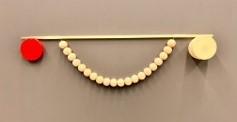
\includegraphics[width=1\textwidth]{papers/kettenlinie/images/kettenlinie_holz.jpg}
		\caption{Kette aus Holz}
		\label{fig:kettenlinie-materialien-holz}
	\end{subfigure}\hfill
	\begin{subfigure}{0.5\textwidth}
		\centering
		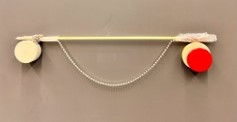
\includegraphics[width=1\textwidth]{papers/kettenlinie/images/kettenlinie_metall.jpg}
		\caption{Kette aus Metall}
		\label{fig:kettenlinie-materialien-metall}
	\end{subfigure}
	\caption{Kettenlinie für Ketten aus verschiedenen Materialien
	\label{fig:kettenlinie-materialien}}
\end{figure}
%
\begin{figure}
	\centering
	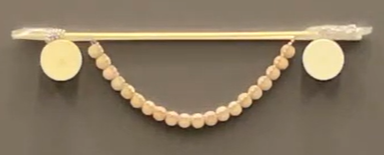
\includegraphics[width=1\textwidth]{papers/kettenlinie/images/kettenlinie_holz_metall.png}
	\caption{Holz-Kettenlinie und Metall-Kettenlinie übereinander gelegt}
	\label{fig:Kettenlinie-Holz-Metall}
\end{figure}
%
Im Abschnitt \ref{kettenlinie:subsection:Minimum der potentiellen Energie} wird hergeleitet, dass die Massendichte ignoriert werden kann. Daraus lässt sich schliessen, dass das Material, aus dem die Kette gefertigt ist, keinen Einfluss auf die Kettenlinie hat.

In den Abbildungen \ref{fig:kettenlinie-materialien}~(a) und
\ref{fig:kettenlinie-materialien}~(b) sind zwei Ketten mit derselben
Länge an zwei Aufhängepunkten mit der gleichen Distanz abgebildet.
Einziger Unterschied sind die verwendeten Materialien.
Die Kette in \ref{fig:kettenlinie-materialien}~(a) ist aus Holzperlen,
wobei in \ref{fig:kettenlinie-materialien}~(b) Metallperlen verwendet
wurden.
Metall und Holz haben eine unterschiedliche Dichte, dennoch ist die
Form der Kettenlinie für beide Ketten immer noch dieselbe, wie in
Abbildung \ref{fig:Kettenlinie-Holz-Metall} zu sehen, wo die beiden
Ketten übereinander gelegt sind.
\index{Metall}%
\index{Holz}%


\subsection{Versuch 2: Kettenlinien in verschiedenen Umgebungen
\label{kettenlinie:subsection:umgebung}}
\begin{figure}
	\centering
	\def\h{2.6}
	\def\w{3.2}
	\def\s{0.2}
	\def\t{0.2}
	\begin{subfigure}{0.50\textwidth}
		\centering
		\begin{tikzpicture}[>=latex,thick]
			\fill[color=white] (-\w,-\h) rectangle (\h,\h);
			\clip ({-\w+\s},{-\h+\t}) rectangle ({\w-\s},{\h-\t});
			\node at (0,0) {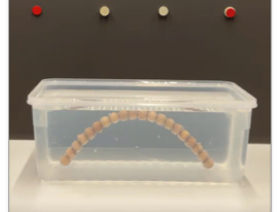
\includegraphics[width=6.4cm]{papers/kettenlinie/images/kettenlinie_holz_wasser.png}};
		\end{tikzpicture}
		\caption{Kette aus Holz im Wasser}
		\label{fig:Kettenlinie-Holz-Wasser}
	\end{subfigure}\hfill
	\begin{subfigure}{0.50\textwidth}
		\centering
		\begin{tikzpicture}[>=latex,thick]
			\fill[color=white] (-\w,-\h) rectangle (\h,\h);
			\clip ({-\w+\s},{-\h+\t}) rectangle ({\w-\s},{\h-\t});
			\node at (0,0) {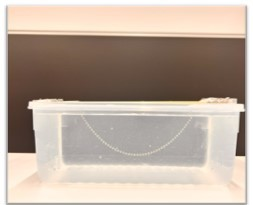
\includegraphics[width=6.4cm]{papers/kettenlinie/images/kettenlinie_metall_wasser.jpg}};
		\end{tikzpicture}
		\caption{Kette aus Metall im Wasser}
		\label{fig:Kettenlinie-Metall-Wasser}
	\end{subfigure}
	\caption{Ketten unter Wasser ergeben die gleiche Kettenlinie unabhängig
	vom Material.
	\label{fig:kettenlinie-wasser}}
\end{figure}
%
\begin{figure}
	\centering
	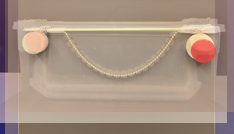
\includegraphics[width=1\textwidth]{papers/kettenlinie/images/kettenlinie_merged.png}
	\caption{Vier Kettenlinien übereinander gelegt}
	\label{fig:Kettenlinie-Merged}
\end{figure}
%
Auch in Abschnitt \ref{kettenlinie:subsection:Minimum der potentiellen Energie} wird die Gravitationskonstante ignoriert.
Da die Gravitation keine Rolle spielt für die Form der Kettenlinie, lässt sich annehmen dass egal in welcher Umgebung die Kette aufgehängt wird, sie immer in derselben Form bleibt.
Wichtig ist nur, dass eine Gravitationskraft existiert.
Um diese Annahme zu testen, werden die Kettenlinien von Versuch 1 im Abschnitt \ref{kettenlinie:subsection:massendichte} wiederverwendet, aber diesmal in Wasser aufgehängt.

In den Abbildungen \ref{fig:kettenlinie-wasser}~(a) und
\ref{fig:kettenlinie-wasser}~(b) sind diese Kettenlinien im Wasser zu sehen.
Legt man diese wieder übereinander, sieht man dass die Form unverändert bleibt.
In Abbildung \ref{fig:Kettenlinie-Merged} wird dies, zusätzlich mit den Kettenlinien aus Versuch 1, nochmal veranschaulicht.

\subsection{Versuch 3: Kettenlinien im Wasser
\label{kettenlinie:subsection:wasser}}

Aus dem vorherigen Versuch, wurden einige Verhaltensänderungen festgestellt.
So entsteht bei der Kette aus Holz eine umgekehrte Kettenlinie im Wasser.
Grund dafür ist natürlich die geringere Dichte von Holz gegenüber von Wasser.
Da die Aufhängepunkte der Kette unter Wasser sind, entsteht durch den Auftrieb eine umgekehrte Kettenlinie.
Diese Kettenlinie hat immer noch dieselbe Form wie die restlichen Kettenlinien in diesem Experiment, jedoch um 180° gedreht.

In der Abbildung \ref{fig:Kettenlinie-Curves} ist eine weitere Besonderheit zu sehen.
\begin{figure}
	\centering
	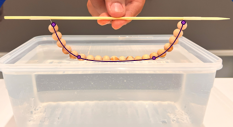
\includegraphics[width=1\textwidth]{papers/kettenlinie/images/kettenlinie_curves.png}
	\caption{Kettenlinie mit Knicke, es entstehen drei Kettenlinien}
	\label{fig:Kettenlinie-Curves}
\end{figure}

Wenn die Holzkettenlinie auf der Wasseroberfläche aufkommt, entstehen durch den Auftrieb Knicke.
Spannend dabei ist, dass dadurch drei Segmente entstehen.
In jedem Segment entsteht zwischen den Knicken eine eigene, neue Kettenlinie.


\subsection{Fazit Experiment
\label{kettenlinie:subsection:fazit-experiment}}
Aus dem Experiment ist klar erkennbar, dass Faktoren wie Materialdichte und Gravitationskräfte keine Auswirkungen auf die Form der jeweiligen Kettenlinie haben.
Die mathematischen Herleitungen stimmen und wurden durch die Experimente auch visuell bewiesen.


\printbibliography[heading=subbibliography]
\end{refsection}
